\subsection{Convolutional Neural Networks}
\label{sec:neural-networks-convolutional-neural-networks}
Convolutional neural networks are suited for image processing tasks, because they perform better than the multilayer perceptrons architecture regarding accuracy and the number of parameters\cite{Lecun98}\cite{LeCun1998cnn}.
The reason for the first one is most likely that they are invariant regarding the position of an object within an image.
Convolutional neural networks do not have a as strict separation in multiple layers as multilayer perceptrons do.
They rather have a pool of several layers which can be arbitrarily connected to fulfill one's needs.

\subsubsection{Convolutional Layer}
\label{sec:cnn-convolutional-layer}
The first convolutional layer in a network usually works directly on the prepared input data for finding features.
As the name suggests it performs a convolution with a filter matrix of arbitrary size on an input matrix of arbitrary size.
The input matrix corresponds to spatial input neurons and is, for example, an image $\vec{I} \in \mathbb{R}^{u \times v}$.
The filter or kernel matrix $\vec{K} \in \mathbb{R}^{i \times j}$ contains $i \cdot j$ weights of the network.
The filter is moved across the neurons and performs a dot product within its window.
Hence, its weights are reused for different areas in the image.
\figref{fig:convolution} illustrates the following operation.
In reference to the figure, the kernel covers the four elements in the top right corner of the input image.
Hence, the dot product multiplication for this setup yields $5 \cdot 1+4 \cdot (-1)+1 \cdot (-1)+3 \cdot 1=3$.
This result is stored in a new matrix $\vec{F}$ at its corresponding place.
In the end, this matrix will hold all values of the convolution operation.
After each calculation of the dot product, the filter matrix moves.
The corresponding step size is called stride.
A stride of $s=1$ moves the filter by one pixel or neuron, respectively.
There can be a different stride along the row and height dimension.
This resulting matrix is called a feature map because it stores the features extracted from the input.
With
\begin{subequations}
	\label{eq:feature-map-shape}
	\begin{align}
		\dim(\vec{F})_1 &= \floor \left( \frac{u - i}{s}+1 \right) \\
		\dim(\vec{F})_2 &= \floor \left( \frac{v - j}{s}+1 \right)
	\end{align}
\end{subequations}
its shape can be calculated.
\begin{figure}
	\centering
	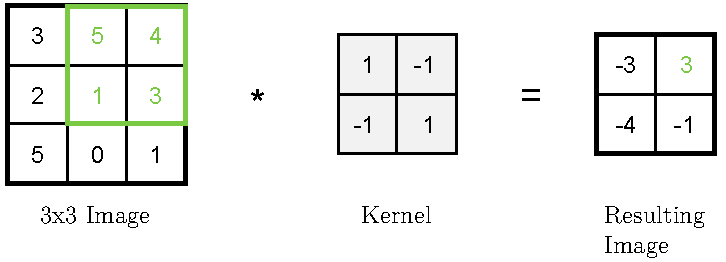
\includegraphics{images/convolution.pdf}
	\caption[Convolution of an image with a kernel]{Convolution of an image $\vec{I}$ with a kernel $\vec{K}$. The $2 \times 2$ kernel is moved across the $3 \times 3$ image and performs a dot product multiplication within its window each time. Here, the kernel moves with a stride of $s=1$, which results in the shown image on the right, the so-called feature map $\vec{F}$.}
	\label{fig:convolution}
\end{figure}
In this operation, the feature map is always smaller than the input, because only convolutions are performed with the filter inside the input.
Sometimes this is not desirable, as it can lead to loss in information in the edge regions.
This is because they are less frequent inside the filter window.
Moreover, if multiple convolutions are performed consecutively, the feature map constantly shrinks, because each convolution operates on the latest feature map, until no feature can be extracted anymore or only few detailed ones.
\begin{figure}
	\centering
	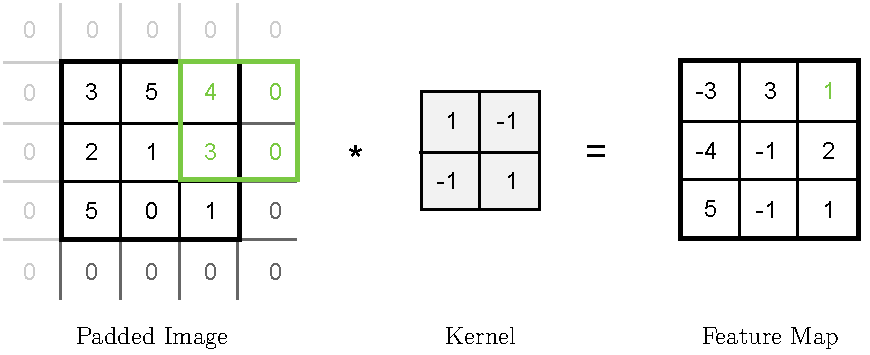
\includegraphics{images/convolution_padding.pdf}
	\caption[Convolution of a padded image with a kernel]{Convolution of a padded image with a $2 \times 2$ kernel $\vec{K}$. The $3 \times 3$ image $\vec{I}$ is surrounded with $p=0.5$ rounds of zeros for yielding a feature map $\vec{F}$ of same size. If the amount of padding is odd, two contiguous sides are preferred.}
	\label{fig:convolution-padding}
\end{figure}
In practical terms, there are two common conventions for convolutions, which are called valid and same in the following.
The former defines that no padding is applied and therefore a valid convolution is performed because only the real input and full kernel windows are taken into account.
This means that the feature map has a size of $\vec{F} \in \mathbb{R}^{\dim(\vec{F})_1 \times \dim(\vec{F})_2}$.
The latter means, that the size of the feature map equals the one of the input.
Thus, a padding $p$ can be applied to the input.
This means surrounding the input with zeros to create a larger input.
The convolution operates like usual, just on a larger input.
How much padding $p$ needs to be applied can be calculated by comparing both matrix shapes.
Therefore, the expression
\begin{subequations}
	\begin{equation}
		u := \frac{u-i+2p}{s}+1
	\end{equation}
needs to be valid, yielding
\begin{equation}
	p = \frac{u(s-1)+i-s}{2}
\end{equation}
\end{subequations}
for calculating the amount of padding on each related side.
However, in general, this only covers the padding height.
If the image or filter are not symmetric, the padding along the width needs to be calculated as well by replacing $u$ with $v$ and $i$ with $j$.
%Another remark is, that in computer vision filter sizes usually are odd.
%There can be two reasons for this.
%First, the filter has a center which helps to tell where exactly the filter points to.
%Second, the padding $p$ is even.
If the amount of padding is odd, it is performed in half rounds around the image where two contiguous sides of the image are preferred like it is shown in \figref{fig:convolution-padding} with the help of transparency.
Only the padding at the right and at the bottom are taken into account for creating a filter matrix with the same shape of the original input.
For three-dimensional inputs, where each matrix along the depth dimension is called channel, a convolution is performed almost identically.
Instead of a kernel with a depth of one as for a two-dimensional input, it is extended to a depth that matches the input yielding $\dim\left(\vec{K}\right)_3 = \dim\left(\vec{I}\right)_3$.
Then a common dot product multiplication is calculated for every input channel with its corresponding filter channel.
This results in a matrix with the depth of the input and filter.
Finally, the resulting depth channels are summed up element-wise which results in a matrix with depth one, i.e. $\dim\left(\vec{F}\right)_3 = 1$.
For the case of an RGB image, that is an image with three channels representing the colors red, green and blue, a filter would have a depth of three and a final convolution result would always have a depth of one.
This example is illustrated in \figref{fig:convolution-channels}.
\begin{figure}
	\centering
	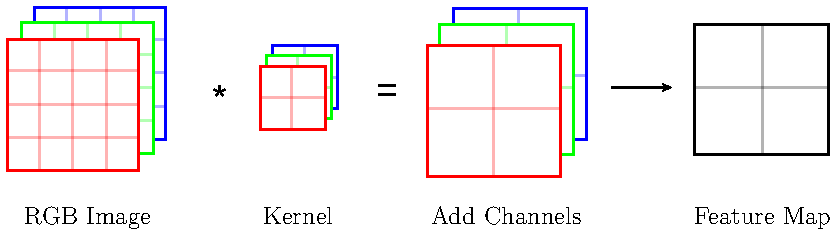
\includegraphics{images/convolution_channel.pdf}
	\caption[Convolution of input with multiple channels]{Convolving an RGB input $\vec{I}$ with $\dim(\vec{I})_3=3$ channels needs a kernel $\vec{K}$ with $\dim(\vec{K})_3 = \dim(\vec{I})_3$. This results in one convolution result per corresponding channels. Those are summed element-wise for yielding a two-dimensional feature map $\vec{F}$.}
	\label{fig:convolution-channels}
\end{figure}
Usually, at the end of a convolutional layer, a bias addition is performed for simulating the neurobiological spike of a neuron.
This result is put into an activation function like the ones from \figref{fig:activation-functions}.
Both the methods and their purposes are analog to the ones known from multilayer perceptron networks.

The kernel in \figref{fig:convolution} would find top-left to bottom-right diagonal lines because its convolution result is higher if the pixels in its window represent such a shape.
For example, there is a black image with white shapes.
If the filter is on a plain surface, where all pixel values have the same intensity, the convolution result is 0 due to the positive and negative weights.
However, if it is over such a line, the result is higher because the pixels representing the line are fully taken into account.
If the line points into the other direction the representing pixels are not taken into account, while the other two are weighted negatively.
Like this but with slightly larger kernels and different weights more complex features can be found.
Finding discriminative features depends on a satisfiable set of weights and biases, though.
It is also possible to perform multiple different convolutions on the same input to find different features.
They are stored as a matrix, where the number of different features represents the depth of the feature map $\vec{F}$.
This whole process solves the limitation to a fixed position of features of the multilayer perceptrons architecture.
Even if, for example, a digit is not centered anymore in the image, all features are found, because the kernel is moved over the image for checking the presence of a certain feature.
Hence, this keeps the spatial relationship of pixels that is lost if an input is flattened as with multilayer-perceptrons networks, where each perceptron is responsible for one single pixel.
Furthermore, because each feature is found by a moving filter, convolutional neural networks need way fewer weights and biases due to the possibility of reusing them for different image areas.
The accuracy compared to multilayer perceptron networks is improved by concatenating several convolutions.
That means a convolution is performed on the activation of an earlier convolution or more generally on the activation of its preceding layer.
This way, first, rough features like edges are found for narrowing down possible classes, and the deeper it gets into the network, the finer the features get.
\subsubsection{Pooling Layer}
\label{sec:cnn-pooling-layer}
After obtaining features using a convolutional layer a pooling layer can be inserted.
Pooling serves as a sample-based discretization process.
This is done by moving a filter with an arbitrary stride over the input that compresses the information or values, respectively, within its window.
The result is a reduction of the inputs spatial dimensions.
However, the depth stays the same.
The objective of this process is a gain in computational performance, because there is less spatial information.
Hence, fewer weights and biases are needed which in turn improves training time.
Another advantage is a less chance for overfitting due to the loss of spatial information.
Moreover, the extracted features are translation invariant.
This means, that features can be found even when they underwent a small positional displacement
The reason for this is, that within the pooling window the found translated feature is still more important than another one
For example, the network classifies perfectly round zeros by looking for four quarter circles as features next to each other.
Though, the input is a wider zero and, thus, the network finds small lines as features between the quarter circle features.
If the pooling window now checks one of these quarter circle features extended with a line feature, still the first feature is used for further calculations because it is more important.
\figref{fig:pooling} illustrates the pooling process for a max pooling operation in practical terms.
A max pooling filter yields the maximum within its window as the result.
Moving such a $2 \times 2$ filter over the $4 \times 4$ input with a stride of $2$ yields a matrix with each maximum at its corresponding position.
The maximum of the red colored $2 \times 2$ window is 7, hence, this number comes up in the result.
The other windows are processed identically.
The size of the result of an arbitrary pooling operation with an input of size $w_1 \times h_1 \times d_1$ and a filter of size $f \times f$ is
\begin{align}
	w_2 &= \frac{w_1 - f}{s}+1 \\
	h_2 &= \frac{h_1 - f}{s}+1 \\
	d_2 &= d_1
\end{align}
where $w$ is the number the rows, $h$ the number of columns, $d$ the depth and $s$ the stride.
As it can be seen, pooling layers do not have learnable parameters only hyperparameters.
There are only two common variations of hyperparameters.
Either $f=3$ and $s=2$, which models a overlapped pooling operations, because some values are part of different windows, or $f=2$ and $s=2$.
Larger filters and strides take away too much information.
Another pooling type is mean pooling.
Hereby, the result of each window is the average of all its values instead of the largest one.
However, its results are outperformed by the max pooling\cite{Scherer2010}.
\begin{figure}
	\centering
	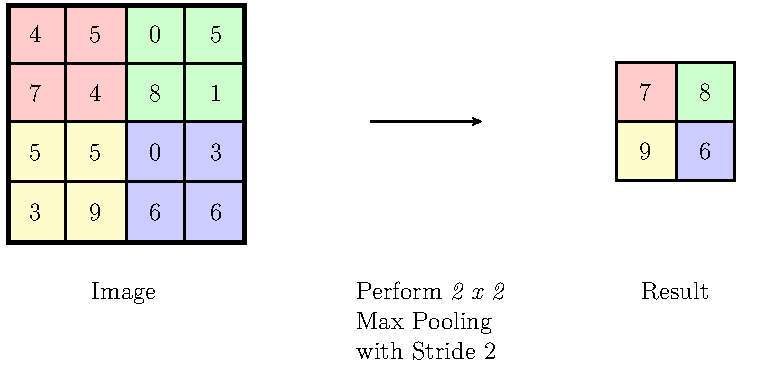
\includegraphics{images/pooling.pdf}
	\caption[Max Pooling with $2 \times 2$ Filter and Stride $2$]{Max pooling with $2 \times 2$ filter across a $4 \times 4$ input with a stride of $2$. Within each window the maximum of its values is computated. Finally, this yiels a matrix with each maximum at its corresponding position.}
	\label{fig:pooling}
\end{figure}
\subsubsection{Fully-Connected Layer}
\label{sec:cnn-fully-connected}
The last part of a convolutional neural network consists of at least one fully connected layer.
This is identical to \figref{fig:multilayer-perceptron} but instead of directly inputting real-world values the output or activations, respectively, of the previous convolutional or pooling layer, is used.
However, fully-connected layers can be stacked, so the outputs of one can be the inputs of another one.
Every edge has a weight and every node has a bias.
The values flowing over an edge are multiplied with the related weight and summed up.
To this weighted sum, the bias of the neuron is added and the result is fed into an activation function.
Describing this in a mathematical sense can be done with \eqref{eq:perceptron-activation}.
The objective is to combine several features that were detected and use them as attributes for classifying the input.
Due to the weights, some attributes are more significant than others.
For example, if four legs and a long nose are found, there is a dog in the image and not a cat.
If the task is to distinguish only between cats and dogs, the nose feature is weighted more than the leg feature.
For preventing overfitting and improving generalization, a fully-connected layer can be combined with the dropout regularization technique\cite{Srivastava:2014:DSW:2627435.2670313}.
This drops out nodes randomly during training depending on a given probability, i.e. changing their incoming and outgoing weights temporarily to zero.
Hence, those nodes are excluded from the current classification and from backpropagation as well.
So their weights experience no change, which achieves the desired effect.
The interpretation of the outputs of a fully connected layer is simplified by applying an additional softmax function that squashes the output into a range of 0 and 1, whereas the sum of all outputs equals 1, to represent percentages of confidence or a probability distribution, respectively\cite{Bishop2006}.
The softmax function can be written as
\begin{equation}
	\label{eq:softmax}
	S(y_i) = \frac{\exp(y_i)}{\sum_{j} \exp(y_j)}
\end{equation}
where $y$ are the outputs, $i$ an index of an output and $j$ a moving index over all outputs.
This exploits the knowledge of mutually exclusive classes, i.e. that only one class is correct.
Otherwise, for multi-label classification, a sigmoid function can be used, that squashes each output of the network into a range of 0 and 1.